\section{Zielsetzung}
Im folgenden Versuch soll das Phänomen der Dispersion mithilfe einer Heliumlampe und eines Glasprismas untersucht werden. Genauer werden in zwei Versuchsteilen verschiedene Winkel bestimmt, aus denen auf das Dispersionsverhalten geschlossen werden kann.

\section{Theorie}
Tritt Licht mit der Lichtgeschwindigkeit $c$ in ein Medium ein, so wechselwirken die Lichtwellen mit den im Medium befindlichen Elektronen, wodurch sich die Geschwindigkeit des Lichtes  zu $v < c$ verringert. Beim Ein- oder Austreten des Lichts in oder aus 
dem Material unter einem Winkel ist ebenso zu beobachten, dass sich die Richtung des Lichtstrahls ändert, was Brechung genannt wird. Eine wichtige Größe, die dies charakterisiert, ist der Brechungsindex $n$, welcher sich aus dem Verhältnis der Lichtgeschwindigkeiten 
in den verschiedenen Medien ergibt:

\begin{equation}
n \:= \frac{v_1}{v_2} = \frac{c}{v}
\end{equation}

Der Brechungsindex kann außerdem auch über zwei Winkel bestimmt werden. Wichtig ist hierbei das Huygenssche Prinzip, das besagt, dass jeder Punkt einer Wellenfront das Zentrum einer neuen Elementarwelle ist. Fällt ein Lichtstrahl unter dem Winkel $\alpha$ gegen 
die Flächennormale auf ein Medium, so kommt es beim Eindringen zu einer Richtungsänderung. Innerhalb des Mediums breitet sich das Licht dann unter dem Winkel $\beta$ aus. 
In Abbildung \ref{fig:huygens} ist zu sehen, dass die Wellenfront zwischen den Punkten A und B im  Punkt A die Grenzfläche der beiden Medien bereits erreicht hat, während Punkt B die Grenzfläche erst nach $T = \frac{\overline{BC}}{v_1}$ erreicht. Nach diesem Zeitraum besitzt die Elemtenarwelle von 
Punkt A den Radius $Tv_2$, der Radius der Elementarwelle im Punkt C ist hingegen noch null. Ab diesem Zeitpunkt entsteht eine Wellenfront zwischen A‘ und C, wobei folgende Beziehungen gelten:

\begin{equation}
\begin{aligned}
\symup{sin}(\alpha) &= \frac{\overline{BC}}{\overline{AC}} = \frac{Tv_1}{\overline{AC}}, \\
\symup{sin}(\beta) &= \frac{\overline{A'A}}{\overline{AC}} = \frac{Tv_2}{\overline{AC}} \\
\end{aligned}
\end{equation}
Hieraus folgt:

\begin{equation}
\frac{\symup{sin}(\alpha)}{\symup{sin}(\beta)} = \frac{v_1}{v_2} = n.
\end{equation}

\begin{figure}[h!tbp]
	\centering
	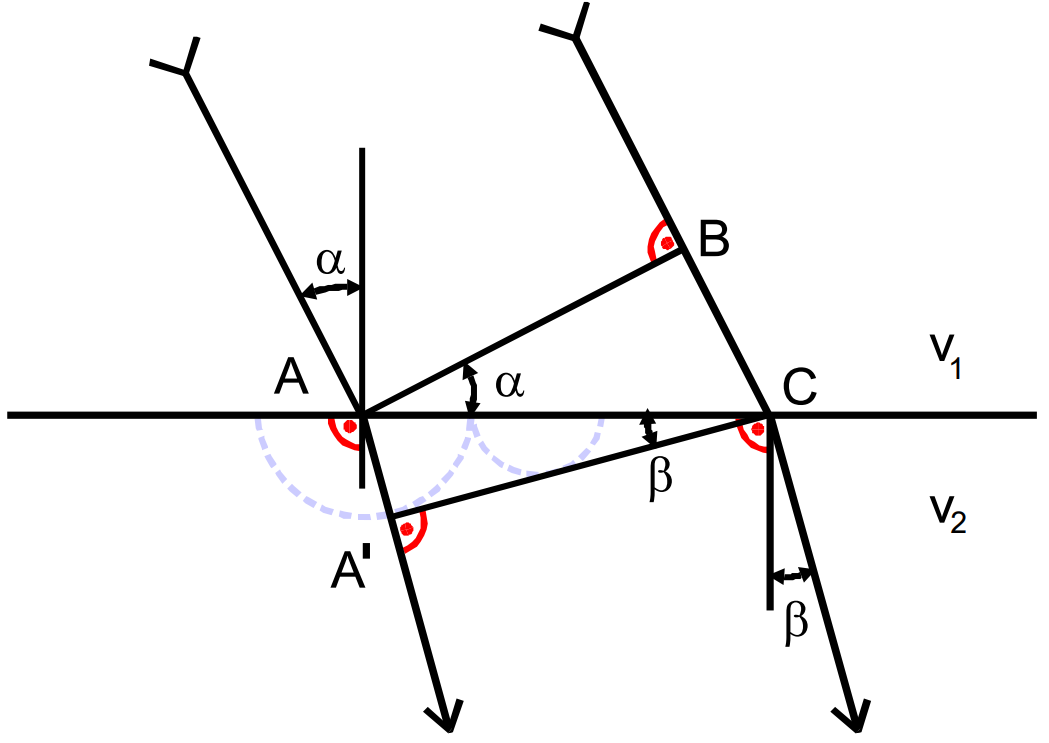
\includegraphics[width=0.7\linewidth]{hyugens}
	\caption{Skizze zum Huygenschen Prinzip, \cite[2]{anleitungV402}.}
	\label{fig:hyugens}
\end{figure}

Weiterhin ist die Geschwindigkeit von Licht in einem Medium von der Frequenz abhängig und somit ist es auch der Brechungsindex $n$. Dieser Zusammenhang wird Dispersion genannt, wobei vor allem die Dispersionskurve der Form:

\begin{equation}
n = f(\lambda)
\end{equation}
wichtig ist. Diese kann mit einem Prisma  gewonnen werden, indem in diesem ein Lichtstrahl zweimal gebrochen wird. 

Zur Ableitung der Dispersionsgleichung werden Elektronen und Ionenrümpfe als Dipole betrachtet, die in dem elektrischen Wechselfeld der Lichtwellen zu schwingen beginnen. Dieses Modell ist nur für den sichtbaren Spektralbereich anwendbar, da die Absorption der Energie des Lichts hier zu vernachlässigen ist,
wohingegen bei Wellenlängen unterhalb des sichtbaren Bereichs Resonanzstellen auftreten, bei denen Absorption stattfindet.
Die einfallende Lichtwelle besitzt eine elektrische Feldstärke von:

\begin{equation}
\vec{E} = \vec{E_0} e^{i\omega t}
\end{equation}
durch die eine periodische Kraft:

\begin{equation}
\vec{F_{\text{e}}} = q_{\text{h}} \vec{E}
\end{equation}
auf die Ladungen $q_{\text{h}}$ ausgeübt wird, wodurch diese sich um $\vec{x_{\text{h}}}$ aus ihrer Gleichgewichtslage verschieben. Dadurch wirkt auf die Ladungen eine rücktreibende Kraft $\vec{F_{\text{r}}}$, die proportional zur Auslenkung ist, sowie auch eine Reibungskraft $\vec{F_{\text{d}}}$, welche
proportional zur Geschwindigkeit der Ladungsträger ist.
Hieraus ergibt sich für die Bewegung der Ladungsteilchen eine Differentialgleichung der Form:

\begin{equation}
m_{\text{h}} \frac{\symup{d}^2\vec{x_{\text{h}}}}{\symup{d}t^2} + f_{\text{h}}\frac{\symup{d}\vec{x_{\text{h}}}}{\symup{d}t} + a_{\text{h}}\vec{x_{\text{h}}} = q_{\text{h}} \vec{E_0} e^{i \omega t}
\end{equation}

Wird die Gleichung mit $\frac{N_{\text{h}} q_{\text{h}}}{m_{\text{h}}}$ erweitert, kann $\vec{x}_{\text{h}}$ durch die Polarisation $\vec{P}_{\text{h}}$ ersetzt werden:

\begin{equation}
\frac{\symup{d}^2\vec{P_{\text{h}}}}{\symup{d}t^2} + \frac{f_{\text{h}}}{m_{\text{h}}}\frac{\symup{d}\vec{P_{\text{h}}}}{\symup{d}t} + \frac{a_{\text{h}}}{m_{\text{h}}}\vec{P_{\text{h}}} = \frac{N_{\text{q}} q_{\text{h}}^2}{m_{\text{h}}} \vec{E_0} e^{i \omega t}.
\end{equation}

Mithilfe der Polarisation $\vec{P}$:

\begin{equation}
\vec{P} = \sum_h \vec{P_{\text{h}}} = \sum_h N_{\text{h}} q_{\text{h}} \vec{x_{\text{h}}}
\end{equation}
und der Maxwellschen Relation $n^2 = \epsilon$  kann nun ein Zusammenhang zwischen Brechungsindex und Lichtfequenz gebildet werden:

\begin{equation}
\tilde{n}^2 = 1 + \sum_h \frac{1}{\omega_{\text{h}}^2 - \omega^2 + i \frac{f_{\text{h}}}{m_{\text{h}}} \omega} \frac{N_{\text{q}} q_{\text{h}}^2}{m_{\text{h}} \epsilon_0}
\end{equation}
Dies lässt sich in einen Real- und einen Imaginärteil aufspalten, woraus sich die Dispersionsgleichungen ergeben. Da die Frequenzen des sichtbaren Lichts relevant sind, wird nur der Bereich betrachtet, der sich weit von den Resonanzstellen entfernt befindet. Hierzu kann 

\begin{equation*}
n^2k \approx 0
\end{equation*}
angenommen werden. Wird nun $\omega$ durch die Wellenlänge $\lambda$ im Vakuum ersetzt, so ergibt sich

\begin{equation}
n^2(\lambda) = 1 + \sum_h \frac{N_{\text{h}} q_{\text{h}}^2}{4\pi^2 c^2 \epsilon_0 m_{\text{h}}} \frac{\lambda^2 \lambda_{\text{h}}^2}{\lambda^2 - \lambda_{\text{h}}^2}.
\label{eq:nquadrat}
\end{equation}
Nun können zwei Fallunterscheidungen vorgenommen werden.

\subsection{Fall: \texorpdfstring{$\lambda$}{Lambda} $>>$ \texorpdfstring{$\lambda_1$}{Lambda_1}}
In dem Fall, dass $\lambda$ viel größer ist als die Absorptionsstelle $\lambda_1$, kann \ref{eq:nquadrat} wie folgt entwickelt werden:

\begin{equation}
\begin{aligned}
\label{eq:gl11}
n^2(\lambda) &= 1 + \frac{N_1 q_1^2 \lambda_1^2}{4 \pi^2 c^2 \epsilon_0 m_1} \biggl(1 + \biggl(\frac{\lambda_1}{\lambda}\biggr)^2 + \biggl(\frac{\lambda_1}{\lambda}\biggr)^4 + ... \biggr) \\
&= A_0 + \frac{A_2}{\lambda^2} + \frac{A_4}{\lambda^4} + ...
\end{aligned}
\end{equation}
mit $A_0$, $A_2$, $A_4 > 0$.


\subsection{Fall: \texorpdfstring{$\lambda$}{Lambda} $<<$ \texorpdfstring{$\lambda_1$}{lambda_1}}
In dem Fall, dass $\lambda$ kleiner ist als die Absorptionsstelle $\lambda_1$, wird aus \ref{eq:nquadrat}:

\begin{equation}
\begin{aligned}
\label{eq:gl12}
n^2(\lambda) &= 1 - \frac{N_1 q_1^2}{4 \pi^2 c^2 \epsilon_0 m_1} \biggl(\lambda^2 + \frac{\lambda^4}{\lambda_1^2} + \frac{\lambda^6}{\lambda_1^4} + ... \biggr) \\
&= 1 - A'_2 \lambda^2 - A'_4 \lambda^4 - ...
\end{aligned}
\end{equation}
mit $A'_{\text{i}} > 0$ für $i \geq 2$.

In Abbildung \ref{fig:dispersionskurven} sind die zugehörigen Kurvenverläufe zu sehen, welche sich durch ihre Krümmung unterscheiden. Genauer gilt bei \ref{eq:gl11}

\begin{equation}
\frac{\symup{d}^2 n^2 (\lambda)}{\symup{d} \lambda^2} > 0
\end{equation}

und im Fall \ref{eq:gl12}
\begin{equation}
\frac{\symup{d}^2n^2(\lambda)}{\symup{d}\lambda^2} < 0.
\end{equation}
Eine Gemeinsamkeit beider Fälle ist, dass es sich um normale Dispersion handelt, was bedeutet, dass der Brechungsindex bei zunehmender Wellenlänge abnimmt. Im Gegensatz dazu bedeutet die anormale Dispersion,
dass der Brechungsindex bei größer werdenen Wellenlängen ebenfalls zunimmt. Die anormale Dispersion ist in diesem Experiment allerdings nicht zu beobachten.

\begin{figure}[h!tbp]
	\centering
	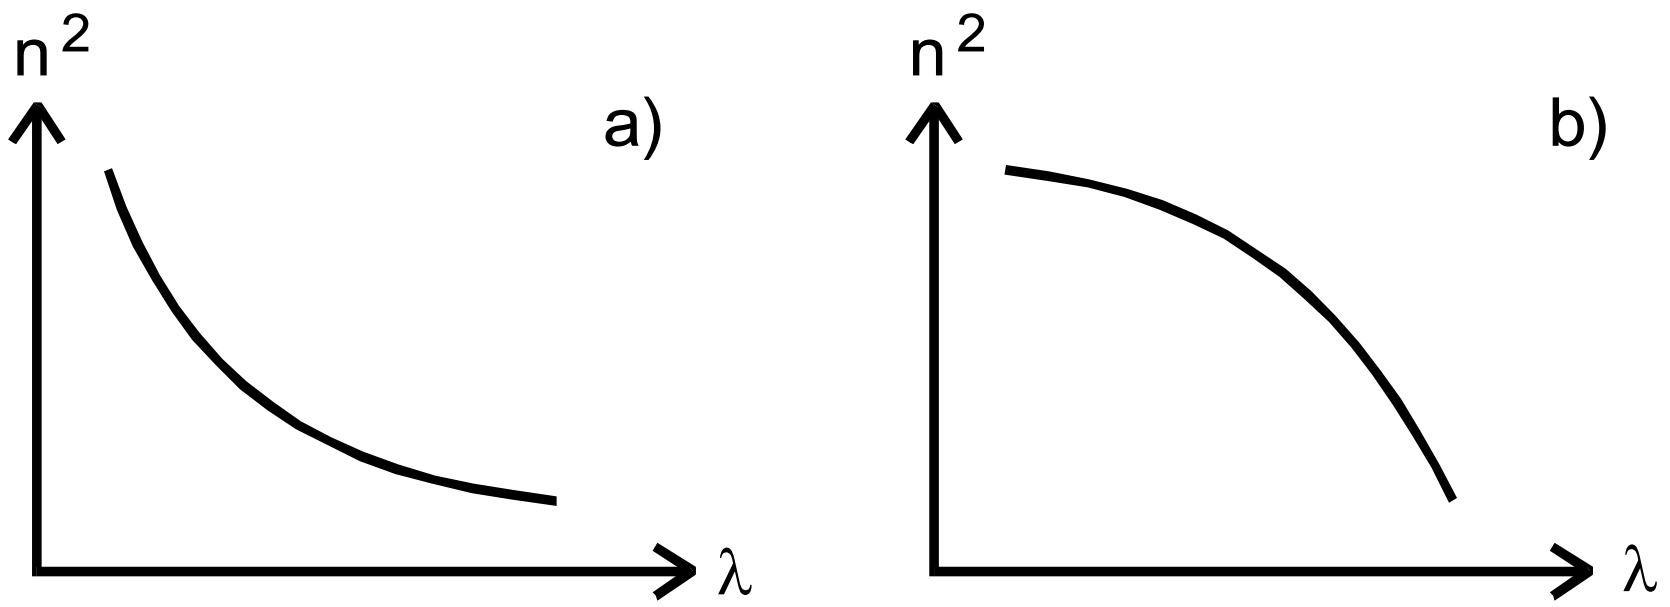
\includegraphics[width=0.7\linewidth]{dispersionskurven}
	\caption{Typische Dispersionskurven, a) nach \ref{eq:fall1}, b) nach \ref{eq:fall2}, \cite[7]{anleitungV402}.}
	\label{fig:dispersionskurven}
\end{figure}

